\section{Evolving Gaussian Processes}
\label{S:active}

In this section, we discuss the challenge of ``Model adaptability" listed in Sec.~\ref{SS:practical_challenges}.

As the system properties change with time, the learned model must actively update itself so that it best reflects the current behavior of the system. %  for best control performance.
For example, the same GP model may not be suitable to control a building in both Summer and Winter seasons.
As we generate more data with time with the controller in the loop, it is intuitive to incorporate the new data into the existing model to improve its accuracy.
However, we may not want to use the full new data set for model update for multiple reasons.
First, because not all data are created equal, especially in closed loop with a controller, we should select only the most informative subset of data that best explain the system dynamics at the time.
Second, since the computational complexity of training and predicting with Gaussian Processes is $\bigO(n^3)$, where $n$ is number of training samples, the learning and control problems become computationally hard as the size of data increases.
Therefore, obtaining the best GP model with the least amount data is highly desired.
The solution to this problem lies in \textit{selecting the optimal subset of data}, from the available data, that best explains the system behavior or dynamics.
Towards this goal, we extend the result from Sec.~\ref{SS:information-theory}.

\subsection{Optimal subset of data selection: selecting the most informative data for periodic model update}

Out goal is to filter the most informative subset of data that best explain the dynamics.
In this section, we outline a systematic procedure that aims to select the best $k$ samples from a given set $\D$ of $n$ observations.
The main differences between the problem of selecting the best or the most informative subset of data and the sequential sampling for OED described in Sec.~\ref{SS:oed:sequential} are that in the former, (1) all the features \(x\) must be optimized as opposed to only control variables \(u\), and (2) the decision has to be made only from the available data rather than sampling. 

We begin by selecting \(k\) samples randomly, %. This is the best result we can obtain using random sampling. We
then assign the priors of the hyperparameters \(\theta\) based on the MLE estimate obtained by learning a GP on the drawn set.
Starting with an empty set of samples \(\mathcal{S}\), %a set \(\mathcal{S}\) consisting of single sample,
we loop through the full data set \(\D\) to identify which sample maximizes the information gain. In this setup, we solve the following optimization problem
\begin{align}
\label{E:oed:batch}
\maximize_{x_{j}|(x_j,y_j) \in \mathcal{D} \setminus \mathcal{S}} & \ \ \ \tilde{\sigma}^2(x_j)/{\sigma}^2(x_j) 
\end{align}
Then, we add this sample to \(\mathcal{S}\), update \(\theta\) and proceed until \(|\mathcal{S}|=k\).
This algorithm is summarized in Algorithm \ref{A:oed:batch}. 

The proposed method is used in a case study in Sec.~\ref{SS:casestudy:active} to update the learned model from time to time as a controller runs in a closed loop and we generate more data.
Fig.~\ref{F:active:example} shows the improvement in mean prediction error and prediction variance obtained after optimal selection, starting with a model trained on uniformly random sampled data. %  using selection based on uniform sampling. 

\begin{algorithm}[!tb]
	\caption{Optimal subset of data selection}
	\label{A:oed:batch}
	\begin{algorithmic}[1]
		\Procedure{Initialization}{}
		\State Sample with replacement \(k\) integers \( \in \{1,\dots,n\} \)
		\State Compute \( \theta_{\mathrm{MLE}} = \argmax_{\theta^{\mathrm{MLE}}} \Pr(Y \vert X, \theta)\)
		\State Assign priors \(\theta_{\mathrm{0}} \sim \GaussianDist{\theta_{\mathrm{MLE}}}{\sigma^2_{\mathrm{init}}}\)
		\EndProcedure
		\State Define \(\mathcal{S} = \varnothing\)
		\Procedure{Sampling}{}
		\While{\( j \leq k \)}
		\State Solve \eqref{E:oed:batch} for optimal \({x_{j} \vert (x_j,y_j) \in \mathcal{D} \setminus \mathcal{S}} \)
		\State \(\mathcal{S} = \mathcal{S} \cup (x_j,y_j) \)
		\State Update \( \theta_{\mathrm{j}} = \argmax_{\theta^{\mathrm{MAP}}} \Pr(Y \vert X, \theta_{\mathrm{j-1}})\)
		\EndWhile
		\EndProcedure
	\end{algorithmic}
\end{algorithm}

\begin{figure*}[t]
	\centering
	\setlength\fwidth{0.37\textwidth} 
	\setlength\hwidth{0.22\textwidth}
	% This file was created by matlab2tikz.
%
%The latest updates can be retrieved from
%  http://www.mathworks.com/matlabcentral/fileexchange/22022-matlab2tikz-matlab2tikz
%where you can also make suggestions and rate matlab2tikz.
%
\definecolor{mycolor1}{rgb}{0.97647,0.89804,1.00000}%
\definecolor{mycolor2}{rgb}{0.85000,0.32500,0.09800}%
%
\begin{tikzpicture}

\begin{axis}[%
width=\fwidth,
height=0.567\hwidth,
at={(0\fwidth,0.387\hwidth)},
scale only axis,
xmin=0,
xmax=95,
xtick={16,32,48,64,80},
xticklabels={\empty},
ymin=0,
ymax=450,
ylabel style={font=\color{white!15!black}},
ylabel={power [kW]},
axis background/.style={fill=white},
xmajorgrids,
ymajorgrids,
legend style={at={(0.5,1.03)}, anchor=south, legend columns=3, legend cell align=left, align=left, fill=none, draw=none},
xlabel style={font=\footnotesize},ylabel style={font=\footnotesize},legend style={font=\footnotesize},ticklabel style={font=\footnotesize},ylabel shift = -5 pt,xlabel shift = -5 pt,
]

\addplot[area legend, draw=mycolor1, fill=mycolor1]
table[row sep=crcr] {%
x	y\\
0	181.797325339693\\
1	165.171361609352\\
2	165.461975867543\\
3	158.175593472448\\
4	163.123829829922\\
5	152.038094910725\\
6	156.776908954676\\
7	157.576424667889\\
8	147.747655912012\\
9	148.456914849296\\
10	154.855162812605\\
11	148.139915337711\\
12	154.989587445275\\
13	175.697416845045\\
14	184.611293252141\\
15	204.930680685881\\
16	215.122488778615\\
17	230.122454391778\\
18	239.871578400889\\
19	272.164405392947\\
20	272.62194164325\\
21	291.631694149582\\
22	312.66123659801\\
23	334.132343852715\\
24	341.925556071999\\
25	341.029804987623\\
26	335.808808011636\\
27	338.041862015376\\
28	318.003544291517\\
29	308.860849680272\\
30	306.950289647017\\
31	289.518164688864\\
32	288.266980777876\\
33	301.615031389896\\
34	280.312311071353\\
35	283.949474393525\\
36	269.051309632789\\
37	276.601021407326\\
38	269.661796010655\\
39	268.371715383921\\
40	265.864839018922\\
41	258.740924958378\\
42	252.055528639332\\
43	252.16821248114\\
44	252.357750043671\\
45	254.252993018447\\
46	261.679297061214\\
47	261.076111309194\\
48	251.954816549178\\
49	244.516939064055\\
50	236.350081099724\\
51	247.002014218353\\
52	246.337699093996\\
53	253.965010231572\\
54	262.165092361783\\
55	279.682247333419\\
56	284.240807614937\\
57	291.890034114044\\
58	287.382919663959\\
59	285.281860909479\\
60	297.026246347602\\
61	302.973805634505\\
62	322.941914850384\\
63	334.986208027307\\
64	324.800935160509\\
65	332.48606102037\\
66	322.290741864057\\
67	338.966059081459\\
68	357.856620527291\\
69	346.32990605598\\
70	347.647505414681\\
71	359.198317061634\\
72	379.093942978983\\
73	386.797393093057\\
74	378.298953074814\\
75	383.316191515727\\
76	385.4138938888\\
77	372.969633304539\\
78	375.891291247109\\
79	357.083876459112\\
80	356.069832914529\\
81	343.526280894915\\
82	332.512010075727\\
83	321.046122927098\\
84	305.263714266148\\
85	291.003333054541\\
86	270.795839459929\\
87	253.606410853124\\
88	236.992650651864\\
89	235.627499775618\\
90	230.954372126972\\
91	238.955382395883\\
92	222.023321770483\\
93	208.37817996681\\
94	185.005191253253\\
95	168.864130304752\\
95	60.9366303455081\\
94	60.6394402594353\\
93	111.960282171114\\
92	116.556460155464\\
91	126.342537148968\\
90	134.569644827294\\
89	139.966505564401\\
88	148.916004401268\\
87	165.017025960049\\
86	179.759082769676\\
85	195.95620631159\\
84	210.258050842148\\
83	222.534600021919\\
82	228.889628950798\\
81	242.852949617714\\
80	253.264219652213\\
79	252.166867728977\\
78	268.315026768372\\
77	263.688456200942\\
76	273.975727546029\\
75	271.329724182597\\
74	270.584610574906\\
73	273.797145819046\\
72	267.737840132515\\
71	258.101273637015\\
70	248.651713834571\\
69	242.997564664254\\
68	239.458429576018\\
67	227.072347017161\\
66	210.026602550218\\
65	208.154756879502\\
64	197.94934897392\\
63	192.140416673644\\
62	179.860182212998\\
61	170.186273344439\\
60	166.273332050943\\
59	159.107733651081\\
58	156.97271295469\\
57	155.073395584752\\
56	149.265995239278\\
55	145.489581218947\\
54	139.006143404302\\
53	137.644558987805\\
52	138.237511241877\\
51	139.097809283365\\
50	141.001809885671\\
49	145.873582610579\\
48	152.112277176693\\
47	155.798953464344\\
46	158.621471109084\\
45	159.880074228147\\
44	159.852594181526\\
43	156.791961334428\\
42	159.07486587949\\
41	165.655075029319\\
40	165.840180919289\\
39	171.844237955616\\
38	175.05182795708\\
37	180.570735597302\\
36	176.259940710547\\
35	191.368034742098\\
34	187.51595949749\\
33	207.400639579116\\
32	200.186958490126\\
31	203.456968694201\\
30	217.478400102915\\
29	215.319574880027\\
28	215.308366419291\\
27	237.769915991391\\
26	226.47263946302\\
25	232.631360973845\\
24	239.255441753369\\
23	234.414577990799\\
22	219.286771854077\\
21	200.212023317069\\
20	182.615723560925\\
19	184.895280950092\\
18	148.925340796061\\
17	135.305922629951\\
16	124.810326447907\\
15	119.23839803474\\
14	96.8919765783725\\
13	86.2791711489792\\
12	52.5313839385344\\
11	43.1721060781072\\
10	55.6480728257789\\
9	51.4970028897104\\
8	50.0150608216301\\
7	60.9219386628864\\
6	54.7342258911099\\
5	49.1438224593801\\
4	55.3499832019105\\
3	57.9915469766029\\
2	58.2516876329222\\
1	63.9102670955031\\
0	71.9201510324973\\
}--cycle;
\addlegendentry{$\mu\text{ }\pm\text{ 2}\sigma$}

\addplot [color=black, dashed]
  table[row sep=crcr]{%
0	126.858738186095\\
1	114.540814352428\\
2	111.856831750233\\
3	108.083570224526\\
4	109.236906515916\\
5	100.590958685053\\
6	105.755567422893\\
7	109.249181665388\\
8	98.881358366821\\
9	99.9769588695033\\
10	105.251617819192\\
11	95.656010707909\\
12	103.760485691905\\
13	130.988293997012\\
14	140.751634915257\\
15	162.08453936031\\
16	169.966407613261\\
17	182.714188510864\\
18	194.398459598475\\
19	228.52984317152\\
20	227.618832602088\\
21	245.921858733325\\
22	265.974004226044\\
23	284.273460921757\\
24	290.590498912684\\
25	286.830582980734\\
26	281.140723737328\\
27	287.905889003384\\
28	266.655955355404\\
29	262.090212280149\\
30	262.214344874966\\
31	246.487566691533\\
32	244.226969634001\\
33	254.507835484506\\
34	233.914135284421\\
35	237.658754567812\\
36	222.655625171668\\
37	228.585878502314\\
38	222.356811983867\\
39	220.107976669768\\
40	215.852509969105\\
41	212.197999993848\\
42	205.565197259411\\
43	204.480086907784\\
44	206.105172112598\\
45	207.066533623297\\
46	210.150384085149\\
47	208.437532386769\\
48	202.033546862936\\
49	195.195260837317\\
50	188.675945492697\\
51	193.049911750859\\
52	192.287605167937\\
53	195.804784609689\\
54	200.585617883042\\
55	212.585914276183\\
56	216.753401427108\\
57	223.481714849398\\
58	222.177816309325\\
59	222.19479728028\\
60	231.649789199273\\
61	236.580039489472\\
62	251.401048531691\\
63	263.563312350475\\
64	261.375142067214\\
65	270.320408949936\\
66	266.158672207138\\
67	283.01920304931\\
68	298.657525051655\\
69	294.663735360117\\
70	298.149609624626\\
71	308.649795349325\\
72	323.415891555749\\
73	330.297269456051\\
74	324.44178182486\\
75	327.322957849162\\
76	329.694810717414\\
77	318.329044752741\\
78	322.10315900774\\
79	304.625372094044\\
80	304.667026283371\\
81	293.189615256315\\
82	280.700819513262\\
83	271.790361474509\\
85	243.479769683066\\
86	225.277461114803\\
87	209.311718406586\\
88	192.954327526566\\
89	187.797002670009\\
90	182.762008477133\\
91	182.648959772426\\
92	169.289890962974\\
93	160.169231068962\\
94	122.822315756344\\
95	114.90038032513\\
};
\addlegendentry{$\mu$}

\addplot [color=mycolor2]
  table[row sep=crcr]{%
0	106.466123573565\\
1	115.337391989545\\
2	125.273158240842\\
3	142.317212701248\\
4	97.2409675530797\\
5	136.389138468029\\
6	150.567045213396\\
7	97.155609988864\\
8	129.072664146571\\
9	129.592067622629\\
10	104.470691768386\\
11	141.921803958905\\
12	139.947187715453\\
13	104.062121822958\\
14	168.3292913586\\
15	145.803205079416\\
16	119.904767428118\\
17	150.453610014193\\
18	242.299430766955\\
19	213.534196081758\\
20	248.687587397972\\
21	248.226682789966\\
22	321.941788706261\\
23	323.314470987785\\
24	326.70568406062\\
25	322.404409925456\\
26	285.181925767642\\
27	267.471592562631\\
28	276.005099360238\\
29	271.609070512374\\
30	240.475491110382\\
31	230.254388991089\\
32	241.735705657432\\
33	244.824063253232\\
34	203.924852289705\\
35	198.575837253726\\
36	204.903210288058\\
37	197.31946623712\\
38	188.390014052418\\
39	203.083415426205\\
40	210.712875972167\\
41	202.570966047695\\
42	200.00617429333\\
43	203.833796077024\\
44	204.411607104079\\
45	205.409072662392\\
46	198.990512872913\\
47	205.303749950728\\
48	186.815427103123\\
49	191.430780243249\\
50	181.848116505017\\
51	176.119906048134\\
52	175.610022311717\\
53	177.74416971062\\
54	184.232930409508\\
55	188.415154825496\\
56	192.849597022108\\
57	193.915907616571\\
58	201.470147087986\\
59	209.974346477716\\
60	205.649874937708\\
61	212.031055162601\\
62	247.140117974841\\
63	252.397817805342\\
64	242.567234990774\\
65	237.674532032872\\
66	292.748039782014\\
67	303.56219592991\\
68	300.393993386262\\
69	289.049580278474\\
70	293.226002939291\\
71	293.221624588051\\
72	303.677136423324\\
73	317.020283864049\\
74	342.727549984237\\
75	367.003363196337\\
76	348.022563824059\\
77	352.45785951852\\
78	328.742421255896\\
79	316.755154907224\\
80	319.008219564211\\
81	319.700395197463\\
82	253.600164774883\\
83	254.789897783855\\
84	257.869408303201\\
85	256.714247242328\\
86	201.275624476964\\
87	180.259665094574\\
88	196.045191371375\\
89	197.134409351331\\
90	171.504709783647\\
91	152.104515780711\\
92	113.57884959615\\
93	156.963587794023\\
94	144.279317956355\\
95	113.909483545478\\
};
\addlegendentry{system}

\end{axis}

\begin{axis}[%
width=\fwidth,
height=0.278\hwidth,
at={(0\fwidth,0\hwidth)},
scale only axis,
xmin=0,
xmax=95,
xtick={16,32,48,64,80},
xticklabels={{4am},{8am},{12pm},{4pm},{8pm}},
ymin=0,
ymax=80,
ytick={ 0, 40, 80},
ylabel style={font=\color{white!15!black}},
ylabel={error [kW]},
axis background/.style={fill=white},
xmajorgrids,
ymajorgrids,
xlabel style={font=\footnotesize},ylabel style={font=\footnotesize},legend style={font=\footnotesize},ticklabel style={font=\footnotesize},ylabel shift = -5 pt,xlabel shift = -5 pt,
]

\addplot[area legend, draw=mycolor1, fill=mycolor1, forget plot]
table[row sep=crcr] {%
x	y\\
0	54.9385871535981\\
1	50.6305472569244\\
2	53.6051441173105\\
3	50.0920232479228\\
4	53.8869233140057\\
5	51.4471362256725\\
6	51.0213415317829\\
7	48.3272430025014\\
8	48.8662975451909\\
9	48.4799559797929\\
10	49.6035449934129\\
11	52.4839046298018\\
12	51.2291017533703\\
13	44.7091228480327\\
14	43.8596583368842\\
15	42.8461413255703\\
16	45.156081165354\\
17	47.4082658809135\\
18	45.4731188024142\\
19	43.6345622214278\\
20	45.0031090411624\\
21	45.7098354162566\\
22	46.6872323719665\\
23	49.8588829309583\\
24	51.335057159315\\
25	54.1992220068887\\
26	54.6680842743081\\
27	50.1359730119925\\
28	51.3475889361129\\
29	46.7706374001223\\
30	44.7359447720511\\
31	43.0305979973317\\
32	44.0400111438752\\
33	47.1071959053902\\
34	46.3981757869314\\
35	46.2907198257135\\
36	46.3956844611208\\
37	48.015142905012\\
38	47.3049840267872\\
39	48.2637387141523\\
40	50.0123290498165\\
41	46.5429249645295\\
42	46.4903313799212\\
43	47.688125573356\\
44	46.2525779310723\\
45	47.1864593951498\\
46	51.5289129760652\\
47	52.638578922425\\
48	49.9212696862424\\
49	49.3216782267379\\
50	47.6741356070262\\
51	53.952102467494\\
52	54.0500939260594\\
53	58.1602256218838\\
54	61.5794744787404\\
55	67.096333057236\\
56	67.4874061878296\\
57	68.408319264646\\
58	65.2051033546346\\
59	63.0870636291992\\
60	65.3764571483291\\
61	66.393766145033\\
62	71.5408663186928\\
63	71.4228956768318\\
64	63.4257930932945\\
65	62.1656520704343\\
66	56.1320696569197\\
67	55.9468560321492\\
68	59.1990954756366\\
69	51.6661706958629\\
70	49.4978957900553\\
71	50.5485217123095\\
72	55.6780514232345\\
73	56.5001236370056\\
74	53.857171249954\\
75	55.9932336665648\\
76	55.7190831713852\\
77	54.6405885517984\\
78	53.7881322393689\\
79	52.4585043650675\\
80	51.402806631158\\
81	50.3366656386005\\
82	51.8111905624647\\
83	49.2557614525896\\
84	47.5028317120004\\
85	47.5235633714753\\
86	45.5183783451266\\
87	44.2946924465374\\
88	44.0383231252982\\
89	47.8304971056085\\
90	48.1923636498393\\
91	56.3064226234575\\
92	52.7334308075097\\
93	48.2089488978481\\
94	62.1828754969088\\
95	53.9637499796222\\
95	0\\
94	0\\
93	0\\
92	0\\
91	0\\
90	0\\
89	0\\
88	0\\
87	0\\
86	0\\
85	0\\
84	0\\
83	0\\
82	0\\
81	0\\
80	0\\
79	0\\
78	0\\
77	0\\
76	0\\
75	0\\
74	0\\
73	0\\
72	0\\
71	0\\
70	0\\
69	0\\
68	0\\
67	0\\
66	0\\
65	0\\
64	0\\
63	0\\
62	0\\
61	0\\
60	0\\
59	0\\
58	0\\
57	0\\
56	0\\
55	0\\
54	0\\
53	0\\
52	0\\
51	0\\
50	0\\
49	0\\
48	0\\
47	0\\
46	0\\
45	0\\
44	0\\
43	0\\
42	0\\
41	0\\
40	0\\
39	0\\
38	0\\
37	0\\
36	0\\
35	0\\
34	0\\
33	0\\
32	0\\
31	0\\
30	0\\
29	0\\
28	0\\
27	0\\
26	0\\
25	0\\
24	0\\
23	0\\
22	0\\
21	0\\
20	0\\
19	0\\
18	0\\
17	0\\
16	0\\
15	0\\
14	0\\
13	0\\
12	0\\
11	0\\
10	0\\
9	0\\
8	0\\
7	0\\
6	0\\
5	0\\
4	0\\
3	0\\
2	0\\
1	0\\
0	0\\
}--cycle;
\addplot [color=mycolor2, forget plot]
  table[row sep=crcr]{%
0	20.3926146125304\\
1	0.796577637117508\\
2	13.4163264906093\\
3	34.2336424767223\\
4	11.9959389628366\\
5	35.7981797829765\\
6	44.8114777905032\\
7	12.0935716765238\\
8	30.19130577975\\
9	29.6151087531257\\
10	0.780926050805803\\
11	46.2657932509959\\
12	36.1867020235483\\
13	26.9261721740539\\
14	27.5776564433433\\
15	16.2813342808944\\
16	50.0616401851431\\
17	32.2605784966713\\
18	47.90097116848\\
19	14.9956470897615\\
20	21.0687547958843\\
21	2.30482405664091\\
22	55.9677844802175\\
23	39.041010066028\\
24	36.115185147936\\
25	35.573826944722\\
26	4.04120203031363\\
27	20.4342964407526\\
28	9.34914400483399\\
29	9.5188582322246\\
30	21.7388537645839\\
31	16.2331777004436\\
32	2.49126397656886\\
33	9.68377223127393\\
34	29.9892829947163\\
35	39.0829173140856\\
36	17.7524148836098\\
37	31.2664122651939\\
38	33.9667979314495\\
39	17.0245612435632\\
40	5.13963399693813\\
41	9.62703394615332\\
42	5.55902296608127\\
43	0.646290830759625\\
44	1.69356500851933\\
45	1.65746096090476\\
46	11.1598712122358\\
47	3.13378243604086\\
48	15.2181197598127\\
49	3.76448059406786\\
50	6.82782898768042\\
51	16.9300057027246\\
52	16.6775828562199\\
53	18.0606148990685\\
54	16.3526874735344\\
55	24.1707594506866\\
56	23.9038044049995\\
57	29.5658072328269\\
58	20.7076692213388\\
59	12.2204508025643\\
60	25.9999142615646\\
61	24.5489843268711\\
62	4.26093055684987\\
63	11.1654945451334\\
64	18.80790707644\\
65	32.6458769170638\\
67	20.5429928806001\\
68	1.73646833460725\\
69	5.61415508164339\\
70	4.92360668533485\\
71	15.4281707612739\\
72	19.738755132425\\
73	13.2769855920021\\
74	18.2857681593769\\
75	39.6804053471751\\
76	18.3277531066445\\
77	34.1288147657792\\
78	6.63926224815549\\
79	12.1297828131797\\
80	14.3411932808402\\
81	26.5107799411484\\
82	27.1006547383794\\
83	17.0004636906535\\
84	0.108525749053058\\
85	13.2344775592623\\
86	24.0018366378387\\
87	29.0520533120123\\
88	3.09086384480912\\
89	9.33740668132191\\
90	11.2572986934858\\
91	30.5444439917146\\
92	55.7110413668236\\
93	3.20564327493921\\
94	21.4570022000109\\
95	0.99089677965226\\
};
\end{axis}
\end{tikzpicture}% \hspace{0.5cm}
	% This file was created by matlab2tikz.
%
%The latest updates can be retrieved from
%  http://www.mathworks.com/matlabcentral/fileexchange/22022-matlab2tikz-matlab2tikz
%where you can also make suggestions and rate matlab2tikz.
%
\definecolor{mycolor1}{rgb}{0.97647,0.89804,1.00000}%
\definecolor{mycolor2}{rgb}{0.85000,0.32500,0.09800}%
%
\begin{tikzpicture}

\begin{axis}[%
width=\fwidth,
height=0.567\hwidth,
at={(0\fwidth,0.387\hwidth)},
scale only axis,
xmin=0,
xmax=95,
xtick={16,32,48,64,80},
xticklabels={\empty},
ymin=0,
ymax=450,
ylabel style={font=\color{white!15!black}},
ylabel={power [kW]},
axis background/.style={fill=white},
xmajorgrids,
ymajorgrids,
legend style={at={(0.5,1.03)}, anchor=south, legend columns=3, legend cell align=left, align=left, fill=none, draw=none},
xlabel style={font=\footnotesize},ylabel style={font=\footnotesize},legend style={font=\footnotesize},ticklabel style={font=\footnotesize},ylabel shift = -5 pt,xlabel shift = -5 pt,
]

\addplot[area legend, draw=mycolor1, fill=mycolor1]
table[row sep=crcr] {%
x	y\\
0	156.660537165989\\
1	179.148282074739\\
2	158.525071724553\\
3	157.903540529554\\
4	149.369603185636\\
5	165.546705999386\\
6	181.694018176103\\
7	156.599588879596\\
8	164.632960404498\\
9	165.426830152663\\
10	166.663025070962\\
11	173.883629470937\\
12	169.994892160576\\
13	182.95057609826\\
14	168.539380070541\\
15	182.502367428316\\
16	182.904159689336\\
17	192.865482223376\\
18	207.816355954145\\
19	266.057324435024\\
20	255.615511422969\\
21	284.735556756987\\
22	310.006181064034\\
23	338.411300455707\\
24	342.897064376424\\
25	338.940235296582\\
26	333.990758843207\\
27	325.674611057957\\
28	312.783172456153\\
29	301.237608315975\\
30	288.006848766701\\
31	269.68239920878\\
32	267.594513240275\\
33	255.229083274168\\
34	266.300542277768\\
35	240.358141481025\\
36	251.152886499468\\
37	242.006428820111\\
38	233.080210764458\\
39	243.888714940089\\
40	259.053671072677\\
41	244.730165289663\\
42	247.815032647197\\
43	250.947063286871\\
44	240.045139730845\\
45	240.975176323568\\
46	248.004780569764\\
47	243.954988924217\\
48	236.243667881774\\
49	224.488541727169\\
50	213.193348491263\\
51	221.115893125767\\
52	216.14674640747\\
53	229.005686927744\\
54	227.950839176533\\
55	236.941940767792\\
56	242.143160560954\\
57	247.919677872832\\
58	241.706254877532\\
59	252.86987227822\\
60	259.989445376855\\
61	277.422433834095\\
62	291.824323231564\\
63	310.064125043851\\
64	312.591301249664\\
65	325.912031654603\\
66	326.719212796636\\
67	356.759787890206\\
68	377.434131478156\\
69	365.013685248684\\
70	367.086240394444\\
71	376.494465900591\\
72	399.790842023359\\
73	405.319664688648\\
74	392.093740734455\\
75	393.387585233415\\
76	380.488875948018\\
77	366.86888004154\\
78	365.970958769731\\
79	341.740855351887\\
80	340.580661749721\\
81	325.704448705776\\
82	307.058448046082\\
83	308.937239391828\\
84	292.025211918188\\
85	283.729839438649\\
86	259.29680671\\
87	247.440437654767\\
88	238.15577184116\\
89	220.164294772733\\
90	217.354572568819\\
91	202.815245731058\\
92	193.44165729127\\
93	195.421550440914\\
94	182.309053754445\\
95	172.702395141978\\
95	93.9855217950095\\
94	92.6364423806\\
93	127.386256192161\\
92	119.714409057597\\
91	121.389166114406\\
90	135.594715459522\\
89	138.734006448387\\
88	157.011958466376\\
87	172.267292870058\\
86	183.565894865745\\
85	210.225930834856\\
84	217.910756672072\\
83	229.526955433263\\
82	231.790815983199\\
81	255.581444283561\\
80	268.257010397926\\
79	271.758417170503\\
78	290.693518582988\\
77	287.838318328988\\
76	297.215336985626\\
75	304.555754684494\\
74	302.319584872389\\
73	303.583427912743\\
72	293.43488530883\\
71	278.915951170461\\
70	276.645705425447\\
69	271.653105236015\\
68	277.27267655445\\
67	270.94569522515\\
66	250.097633213593\\
65	246.8348986542\\
64	230.736938538556\\
63	231.942521986713\\
62	222.630276694717\\
61	205.167258174519\\
60	187.973724241432\\
59	181.853797592612\\
58	169.537318970389\\
57	170.946371412078\\
56	164.194323001373\\
55	156.522353618022\\
54	149.216353529481\\
53	143.346008908756\\
52	141.505340637271\\
51	133.56875021628\\
50	148.121469725277\\
49	158.714844489901\\
48	166.800128018336\\
47	175.492947696332\\
46	177.801892983538\\
45	175.237187613577\\
44	171.58126364379\\
43	177.233990016321\\
42	177.691827723414\\
41	175.267130163604\\
40	179.648345109537\\
39	173.168583180446\\
38	157.633899647726\\
37	173.313793603935\\
36	175.100526608388\\
35	165.856608005895\\
34	185.714252782187\\
33	171.886751749237\\
32	193.473923399768\\
31	197.636536954354\\
30	213.655728117857\\
29	231.475286110755\\
28	239.851886373898\\
27	253.65902674802\\
26	257.735726070665\\
25	265.01886031288\\
24	267.205187983189\\
23	264.553600261233\\
22	242.746367108499\\
21	223.453449523244\\
20	192.116087131695\\
19	199.361864836948\\
18	134.879036981067\\
17	112.330892241496\\
16	111.301264735747\\
15	117.707920787561\\
14	101.270345523683\\
13	117.927610051173\\
12	86.1811561636703\\
11	96.5734611429316\\
10	96.6807338239\\
9	99.3109133999954\\
8	95.9888356037088\\
7	93.1366902498411\\
6	109.579644886148\\
5	95.4521833656617\\
4	73.7422769313787\\
3	90.1308526366127\\
2	79.7738561792096\\
1	102.83000413993\\
0	71.1670158508008\\
}--cycle;
\addlegendentry{$\mu\text{ }\pm\text{ 2}\sigma$}

\addplot [color=black, dashed]
  table[row sep=crcr]{%
0	113.913776508395\\
1	140.989143107334\\
2	119.149463951881\\
3	124.017196583083\\
4	111.555940058507\\
5	130.499444682524\\
6	145.636831531125\\
7	124.868139564719\\
8	130.310898004103\\
9	132.368871776329\\
10	131.671879447431\\
11	135.228545306935\\
12	128.088024162123\\
13	150.439093074717\\
14	134.904862797112\\
15	150.105144107938\\
16	147.102712212542\\
17	152.598187232436\\
18	171.347696467606\\
19	232.709594635986\\
20	223.865799277332\\
21	254.094503140115\\
22	276.376274086266\\
23	301.48245035847\\
24	305.051126179807\\
25	301.979547804731\\
27	289.666818902988\\
28	276.317529415025\\
29	266.356447213365\\
30	250.831288442279\\
31	233.659468081567\\
32	230.534218320021\\
33	213.557917511702\\
34	226.007397529977\\
35	203.10737474346\\
36	213.126706553928\\
37	207.660111212023\\
38	195.357055206092\\
39	208.528649060267\\
40	219.351008091107\\
41	209.998647726633\\
42	212.753430185305\\
43	214.090526651596\\
44	205.813201687318\\
45	208.106181968572\\
46	212.903336776651\\
47	209.723968310275\\
48	201.521897950055\\
49	191.601693108535\\
50	180.65740910827\\
51	177.342321671024\\
52	178.82604352237\\
53	186.17584791825\\
54	188.583596353007\\
55	196.732147192907\\
56	203.168741781164\\
57	209.433024642455\\
58	205.621786923961\\
59	217.361834935416\\
60	223.981584809143\\
61	241.294846004307\\
62	257.22729996314\\
63	271.003323515282\\
64	271.66411989411\\
65	286.373465154402\\
66	288.408423005114\\
67	313.852741557678\\
68	327.353404016303\\
69	318.33339524235\\
70	321.865972909945\\
71	327.705208535526\\
72	346.612863666094\\
73	354.451546300695\\
74	347.206662803422\\
75	348.971669958955\\
76	338.852106466822\\
77	327.353599185264\\
78	328.33223867636\\
79	306.749636261195\\
80	304.418836073824\\
81	290.642946494668\\
82	269.424632014641\\
83	269.232097412545\\
84	254.96798429513\\
85	246.977885136752\\
86	221.431350787872\\
87	209.853865262412\\
88	197.583865153768\\
89	179.44915061056\\
90	176.47464401417\\
91	162.102205922732\\
92	156.578033174433\\
93	161.403903316537\\
94	137.472748067522\\
95	133.343958468494\\
};
\addlegendentry{$\mu$}

\addplot [color=mycolor2]
  table[row sep=crcr]{%
0	106.466123573565\\
1	115.337391989545\\
2	125.273158240842\\
3	142.317212701248\\
4	97.2409675530797\\
5	136.389138468029\\
6	150.567045213396\\
7	97.155609988864\\
8	129.072664146571\\
9	129.592067622629\\
10	104.470691768386\\
11	141.921803958905\\
12	139.947187715453\\
13	104.062121822958\\
14	168.3292913586\\
15	145.803205079416\\
16	119.904767428118\\
17	150.453610014193\\
18	242.299430766955\\
19	213.534196081758\\
20	248.687587397972\\
21	248.226682789966\\
22	321.941788706261\\
23	323.314470987785\\
24	326.70568406062\\
25	322.404409925456\\
26	285.181925767642\\
27	267.471592562631\\
28	276.005099360238\\
29	271.609070512374\\
30	240.475491110382\\
31	230.254388991089\\
32	241.735705657432\\
33	244.824063253232\\
34	203.924852289705\\
35	198.575837253726\\
36	204.903210288058\\
37	197.31946623712\\
38	188.390014052418\\
39	203.083415426205\\
40	210.712875972167\\
41	202.570966047695\\
42	200.00617429333\\
43	203.833796077024\\
44	204.411607104079\\
45	205.409072662392\\
46	198.990512872913\\
47	205.303749950728\\
48	186.815427103123\\
49	191.430780243249\\
50	181.848116505017\\
51	176.119906048134\\
52	175.610022311717\\
53	177.74416971062\\
54	184.232930409508\\
55	188.415154825496\\
56	192.849597022108\\
57	193.915907616571\\
58	201.470147087986\\
59	209.974346477716\\
60	205.649874937708\\
61	212.031055162601\\
62	247.140117974841\\
63	252.397817805342\\
64	242.567234990774\\
65	237.674532032872\\
66	292.748039782014\\
67	303.56219592991\\
68	300.393993386262\\
69	289.049580278474\\
70	293.226002939291\\
71	293.221624588051\\
72	303.677136423324\\
73	317.020283864049\\
74	342.727549984237\\
75	367.003363196337\\
76	348.022563824059\\
77	352.45785951852\\
78	328.742421255896\\
79	316.755154907224\\
80	319.008219564211\\
81	319.700395197463\\
82	253.600164774883\\
83	254.789897783855\\
84	257.869408303201\\
85	256.714247242328\\
86	201.275624476964\\
87	180.259665094574\\
88	196.045191371375\\
89	197.134409351331\\
90	171.504709783647\\
91	152.104515780711\\
92	113.57884959615\\
93	156.963587794023\\
94	144.279317956355\\
95	113.909483545478\\
};
\addlegendentry{system}

\end{axis}

\begin{axis}[%
width=\fwidth,
height=0.278\hwidth,
at={(0\fwidth,0\hwidth)},
scale only axis,
xmin=0,
xmax=95,
xtick={16,32,48,64,80},
xticklabels={{4am},{8am},{12pm},{4pm},{8pm}},
ymin=0,
ymax=80,
ytick={ 0, 40, 80},
ylabel style={font=\color{white!15!black}},
ylabel={error [kW]},
axis background/.style={fill=white},
xmajorgrids,
ymajorgrids,
xlabel style={font=\footnotesize},ylabel style={font=\footnotesize},legend style={font=\footnotesize},ticklabel style={font=\footnotesize},ylabel shift = -5 pt,xlabel shift = -5 pt,
]

\addplot[area legend, draw=mycolor1, fill=mycolor1, forget plot]
table[row sep=crcr] {%
x	y\\
0	42.7467606575941\\
1	38.1591389674044\\
2	39.3756077726716\\
3	33.8863439464705\\
4	37.8136631271287\\
5	35.047261316862\\
6	36.0571866449771\\
7	31.7314493148775\\
8	34.3220624003946\\
9	33.0579583763336\\
10	34.9911456235309\\
11	38.6550841640029\\
12	41.906867998453\\
13	32.5114830235438\\
14	33.6345172734291\\
15	32.3972233203772\\
16	35.8014474767945\\
17	40.2672949909401\\
18	36.4686594865393\\
19	33.3477297990381\\
20	31.749712145637\\
21	30.6410536168718\\
22	33.6299069777672\\
23	36.9288500972372\\
24	37.8459381966174\\
25	36.9606874918507\\
26	38.1275163862711\\
27	36.0077921549684\\
28	36.4656430411275\\
29	34.8811611026101\\
30	37.1755603244222\\
31	36.0229311272128\\
32	37.0602949202537\\
33	41.6711657624657\\
34	40.2931447477903\\
35	37.250766737565\\
36	38.0261799455401\\
37	34.3463176080876\\
38	37.7231555583656\\
39	35.3600658798215\\
40	39.7026629815697\\
41	34.7315175630296\\
42	35.0616024618917\\
43	36.8565366352748\\
44	34.2319380435278\\
45	32.8689943549954\\
46	35.101443793113\\
47	34.2310206139422\\
48	34.7217699317189\\
49	32.8868486186339\\
50	32.5359393829929\\
51	43.7735714547437\\
52	37.3207028850996\\
53	42.829839009494\\
54	39.367242823526\\
55	40.2097935748853\\
56	38.9744187797906\\
57	38.486653230377\\
58	36.0844679535717\\
59	35.5080373428042\\
60	36.0078605677115\\
61	36.1275878297884\\
62	34.5970232684234\\
63	39.0608015285691\\
64	40.9271813555541\\
65	39.5385665002015\\
66	38.3107897915214\\
67	42.9070463325278\\
68	50.0807274618533\\
69	46.6802900063344\\
70	45.2202674844986\\
71	48.7892573650649\\
72	53.1779783572646\\
73	50.8681183879524\\
74	44.8870779310329\\
75	44.4159152744603\\
76	41.636769481196\\
77	39.5152808562758\\
78	37.6387200933712\\
79	34.9912190906919\\
80	36.1618256758975\\
81	35.0615022111076\\
82	37.6338160314413\\
83	39.7051419792825\\
84	37.0572276230583\\
85	36.7519543018969\\
86	37.8654559221274\\
87	37.5865723923544\\
88	40.571906687392\\
89	40.715144162173\\
90	40.8799285546482\\
91	40.7130398083257\\
92	36.8636241168367\\
93	34.0176471243761\\
94	44.8363056869224\\
95	39.3584366734842\\
95	0\\
94	0\\
93	0\\
92	0\\
91	0\\
90	0\\
89	0\\
88	0\\
87	0\\
86	0\\
85	0\\
84	0\\
83	0\\
82	0\\
81	0\\
80	0\\
79	0\\
78	0\\
77	0\\
76	0\\
75	0\\
74	0\\
73	0\\
72	0\\
71	0\\
70	0\\
69	0\\
68	0\\
67	0\\
66	0\\
65	0\\
64	0\\
63	0\\
62	0\\
61	0\\
60	0\\
59	0\\
58	0\\
57	0\\
56	0\\
55	0\\
54	0\\
53	0\\
52	0\\
51	0\\
50	0\\
49	0\\
48	0\\
47	0\\
46	0\\
45	0\\
44	0\\
43	0\\
42	0\\
41	0\\
40	0\\
39	0\\
38	0\\
37	0\\
36	0\\
35	0\\
34	0\\
33	0\\
32	0\\
31	0\\
30	0\\
29	0\\
28	0\\
27	0\\
26	0\\
25	0\\
24	0\\
23	0\\
22	0\\
21	0\\
20	0\\
19	0\\
18	0\\
17	0\\
16	0\\
15	0\\
14	0\\
13	0\\
12	0\\
11	0\\
10	0\\
9	0\\
8	0\\
7	0\\
6	0\\
5	0\\
4	0\\
3	0\\
2	0\\
1	0\\
0	0\\
}--cycle;
\addplot [color=mycolor2, forget plot]
  table[row sep=crcr]{%
0	7.44765293482995\\
1	25.6517511177894\\
2	6.12369428896082\\
3	18.3000161181648\\
4	14.3149725054277\\
5	5.88969378550536\\
6	4.93021368227056\\
7	27.7125295758546\\
8	1.23823385753246\\
9	2.77680415369994\\
10	27.2011876790449\\
11	6.69325865197047\\
12	11.8591635533297\\
13	46.3769712517587\\
14	33.4244285614883\\
15	4.30193902852241\\
16	27.1979447844236\\
17	2.14457721824269\\
18	70.9517342993491\\
19	19.1753985542281\\
20	24.8217881206403\\
21	5.86782035014943\\
22	45.5655146199947\\
23	21.832020629315\\
24	21.6545578808132\\
25	20.424862120725\\
26	10.6813166892939\\
27	22.1952263403571\\
28	0.312430054787455\\
29	5.25262329900863\\
30	10.3557973318968\\
31	3.40507909047827\\
32	11.2014873374108\\
33	31.2661457415297\\
34	22.0825452402723\\
35	4.53153748973375\\
36	8.22349626587018\\
37	10.3406449749031\\
38	6.96704115367407\\
39	5.44523363406242\\
40	8.63813211893989\\
41	7.42768167893814\\
42	12.7472558919755\\
43	10.2567305745719\\
44	1.40159458323851\\
45	2.69710930618032\\
46	13.9128239037379\\
47	4.42021835954665\\
48	14.7064708469317\\
49	0.170912865286198\\
50	1.19070739674729\\
51	1.22241562288963\\
52	3.21602121065337\\
53	8.43167820762969\\
54	4.35066594349928\\
55	8.31699236741085\\
56	10.3191447590555\\
57	15.5171170258843\\
58	4.15163983597455\\
59	7.38748845770007\\
61	29.2637908417059\\
62	10.0871819882992\\
63	18.6055057099403\\
64	29.0968849033361\\
65	48.6989331215297\\
66	4.3396167768995\\
67	10.2905456277683\\
68	26.9594106300411\\
69	29.2838149638758\\
70	28.6399699706544\\
71	34.483583947475\\
72	42.9357272427702\\
73	37.4312624366463\\
74	4.47911281918545\\
75	18.0316932373823\\
76	9.17045735723661\\
77	25.1042603332563\\
78	0.410182579536297\\
79	10.0055186460287\\
80	14.5893834903871\\
81	29.0574487027945\\
82	15.8244672397578\\
83	14.4421996286903\\
84	2.90142400807116\\
85	9.73636210557555\\
86	20.1557263109083\\
87	29.5942001678384\\
88	1.53867378239312\\
89	17.685258740771\\
90	4.96993423052339\\
91	9.9976901420211\\
92	42.9991835782833\\
93	4.44031552251445\\
94	6.80656988883263\\
95	19.4344749230157\\
};
\end{axis}
\end{tikzpicture}%
	\caption{Left: Selection using random sampling. Right: Optimal subset of data selection. Starting with the model parameters obtained using random sampling, we apply Algorithm \ref{A:oed:batch} to improve the model accuracy. Both the mean prediction error and the prediction variance are lower for optimal selection based on information gain. }
	\captionsetup{justification=centering}
    \vspace{-10pt}    
	\label{F:active:example}
\end{figure*}


%\begin{figure}[!tb]
%	\centering
%	\setlength\fwidth{0.4\textwidth}
%	\setlength\hwidth{0.3\textwidth}	
%	% This file was created by matlab2tikz.
%
%The latest updates can be retrieved from
%  http://www.mathworks.com/matlabcentral/fileexchange/22022-matlab2tikz-matlab2tikz
%where you can also make suggestions and rate matlab2tikz.
%
\definecolor{mycolor1}{rgb}{0.97647,0.89804,1.00000}%
\definecolor{mycolor2}{rgb}{0.85000,0.32500,0.09800}%
\definecolor{mycolor3}{rgb}{0.92900,0.69400,0.12500}%
%
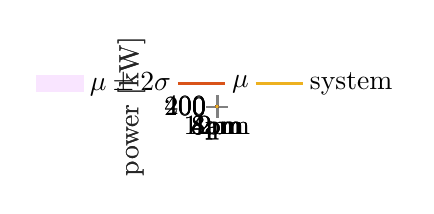
\begin{tikzpicture}

\begin{axis}[%
width=0.951\fwidth,
height=0.419\hwidth,
at={(0\fwidth,0.581\hwidth)},
scale only axis,
xmin=0,
xmax=95,
xtick={16,32,48,64,80},
xticklabels={{4am},{8am},{12pm},{4pm},{8pm}},
ymin=0,
ymax=450,
ylabel style={font=\color{white!15!black}},
ylabel={power [kW]},
axis background/.style={fill=white},
xmajorgrids,
ymajorgrids,
legend style={at={(0.5,1.03)}, anchor=south, legend columns=3, legend cell align=left, align=left, fill=none, draw=none}
]

\addplot[area legend, draw=mycolor1, fill=mycolor1]
table[row sep=crcr] {%
x	y\\
0	156.660537165989\\
1	179.148282074739\\
2	158.525071724553\\
3	157.903540529554\\
4	149.369603185636\\
5	165.546705999386\\
6	181.694018176103\\
7	156.599588879596\\
8	164.632960404498\\
9	165.426830152663\\
10	166.663025070962\\
11	173.883629470937\\
12	169.994892160576\\
13	182.95057609826\\
14	168.539380070541\\
15	182.502367428316\\
16	182.904159689336\\
17	192.865482223376\\
18	207.816355954145\\
19	266.057324435024\\
20	255.615511422969\\
21	284.735556756987\\
22	310.006181064034\\
23	338.411300455707\\
24	342.897064376424\\
25	338.940235296582\\
26	333.990758843207\\
27	325.674611057957\\
28	312.783172456153\\
29	301.237608315975\\
30	288.006848766701\\
31	269.68239920878\\
32	267.594513240275\\
33	255.229083274168\\
34	266.300542277768\\
35	240.358141481025\\
36	251.152886499468\\
37	242.006428820111\\
38	233.080210764458\\
39	243.888714940089\\
40	259.053671072677\\
41	244.730165289663\\
42	247.815032647197\\
43	250.947063286871\\
44	240.045139730845\\
45	240.975176323568\\
46	248.004780569764\\
47	243.954988924217\\
48	236.243667881774\\
49	224.488541727169\\
50	213.193348491263\\
51	221.115893125767\\
52	216.14674640747\\
53	229.005686927744\\
54	227.950839176533\\
55	236.941940767792\\
56	242.143160560954\\
57	247.919677872832\\
58	241.706254877532\\
59	252.86987227822\\
60	259.989445376855\\
61	277.422433834095\\
62	291.824323231564\\
63	310.064125043851\\
64	312.591301249664\\
65	325.912031654603\\
66	326.719212796636\\
67	356.759787890206\\
68	377.434131478156\\
69	365.013685248684\\
70	367.086240394444\\
71	376.494465900591\\
72	399.790842023359\\
73	405.319664688648\\
74	392.093740734455\\
75	393.387585233415\\
76	380.488875948018\\
77	366.86888004154\\
78	365.970958769731\\
79	341.740855351887\\
80	340.580661749721\\
81	325.704448705776\\
82	307.058448046082\\
83	308.937239391828\\
84	292.025211918188\\
85	283.729839438649\\
86	259.29680671\\
87	247.440437654767\\
88	238.15577184116\\
89	220.164294772733\\
90	217.354572568819\\
91	202.815245731058\\
92	193.44165729127\\
93	195.421550440914\\
94	182.309053754445\\
95	172.702395141978\\
95	93.9855217950095\\
94	92.6364423806\\
93	127.386256192161\\
92	119.714409057597\\
91	121.389166114406\\
90	135.594715459522\\
89	138.734006448387\\
88	157.011958466376\\
87	172.267292870058\\
86	183.565894865745\\
85	210.225930834856\\
84	217.910756672072\\
83	229.526955433263\\
82	231.790815983199\\
81	255.581444283561\\
80	268.257010397926\\
79	271.758417170503\\
78	290.693518582988\\
77	287.838318328988\\
76	297.215336985626\\
75	304.555754684494\\
74	302.319584872389\\
73	303.583427912743\\
72	293.43488530883\\
71	278.915951170461\\
70	276.645705425447\\
69	271.653105236015\\
68	277.27267655445\\
67	270.94569522515\\
66	250.097633213593\\
65	246.8348986542\\
64	230.736938538556\\
63	231.942521986713\\
62	222.630276694717\\
61	205.167258174519\\
60	187.973724241432\\
59	181.853797592612\\
58	169.537318970389\\
57	170.946371412078\\
56	164.194323001373\\
55	156.522353618022\\
54	149.216353529481\\
53	143.346008908756\\
52	141.505340637271\\
51	133.56875021628\\
50	148.121469725277\\
49	158.714844489901\\
48	166.800128018336\\
47	175.492947696332\\
46	177.801892983538\\
45	175.237187613577\\
44	171.58126364379\\
43	177.233990016321\\
42	177.691827723414\\
41	175.267130163604\\
40	179.648345109537\\
39	173.168583180446\\
38	157.633899647726\\
37	173.313793603935\\
36	175.100526608388\\
35	165.856608005895\\
34	185.714252782187\\
33	171.886751749237\\
32	193.473923399768\\
31	197.636536954354\\
30	213.655728117857\\
29	231.475286110755\\
28	239.851886373898\\
27	253.65902674802\\
26	257.735726070665\\
25	265.01886031288\\
24	267.205187983189\\
23	264.553600261233\\
22	242.746367108499\\
21	223.453449523244\\
20	192.116087131695\\
19	199.361864836948\\
18	134.879036981067\\
17	112.330892241496\\
16	111.301264735747\\
15	117.707920787561\\
14	101.270345523683\\
13	117.927610051173\\
12	86.1811561636703\\
11	96.5734611429316\\
10	96.6807338239\\
9	99.3109133999954\\
8	95.9888356037088\\
7	93.1366902498411\\
6	109.579644886148\\
5	95.4521833656617\\
4	73.7422769313787\\
3	90.1308526366127\\
2	79.7738561792096\\
1	102.83000413993\\
0	71.1670158508008\\
}--cycle;
\addlegendentry{$\mu\text{ }\pm\text{ 2}\sigma$}

\addplot [color=mycolor2, line width=1.0pt]
  table[row sep=crcr]{%
0	113.913776508395\\
1	140.989143107334\\
2	119.149463951881\\
3	124.017196583083\\
4	111.555940058507\\
5	130.499444682524\\
6	145.636831531125\\
7	124.868139564719\\
8	130.310898004103\\
9	132.368871776329\\
10	131.671879447431\\
11	135.228545306935\\
12	128.088024162123\\
13	150.439093074717\\
14	134.904862797112\\
15	150.105144107938\\
16	147.102712212542\\
17	152.598187232436\\
18	171.347696467606\\
19	232.709594635986\\
20	223.865799277332\\
21	254.094503140115\\
22	276.376274086266\\
23	301.48245035847\\
24	305.051126179807\\
25	301.979547804731\\
27	289.666818902988\\
28	276.317529415025\\
29	266.356447213365\\
30	250.831288442279\\
31	233.659468081567\\
32	230.534218320021\\
33	213.557917511702\\
34	226.007397529977\\
35	203.10737474346\\
36	213.126706553928\\
37	207.660111212023\\
38	195.357055206092\\
39	208.528649060267\\
40	219.351008091107\\
41	209.998647726633\\
42	212.753430185305\\
43	214.090526651596\\
44	205.813201687318\\
45	208.106181968572\\
46	212.903336776651\\
47	209.723968310275\\
48	201.521897950055\\
49	191.601693108535\\
50	180.65740910827\\
51	177.342321671024\\
52	178.82604352237\\
53	186.17584791825\\
54	188.583596353007\\
55	196.732147192907\\
56	203.168741781164\\
57	209.433024642455\\
58	205.621786923961\\
59	217.361834935416\\
60	223.981584809143\\
61	241.294846004307\\
62	257.22729996314\\
63	271.003323515282\\
64	271.66411989411\\
65	286.373465154402\\
66	288.408423005114\\
67	313.852741557678\\
68	327.353404016303\\
69	318.33339524235\\
70	321.865972909945\\
71	327.705208535526\\
72	346.612863666094\\
73	354.451546300695\\
74	347.206662803422\\
75	348.971669958955\\
76	338.852106466822\\
77	327.353599185264\\
78	328.33223867636\\
79	306.749636261195\\
80	304.418836073824\\
81	290.642946494668\\
82	269.424632014641\\
83	269.232097412545\\
84	254.96798429513\\
85	246.977885136752\\
86	221.431350787872\\
87	209.853865262412\\
88	197.583865153768\\
89	179.44915061056\\
90	176.47464401417\\
91	162.102205922732\\
92	156.578033174433\\
93	161.403903316537\\
94	137.472748067522\\
95	133.343958468494\\
};
\addlegendentry{$\mu$}

\addplot [color=mycolor3, line width=1.0pt]
  table[row sep=crcr]{%
0	106.466123573565\\
1	115.337391989545\\
2	125.273158240842\\
3	142.317212701248\\
4	97.2409675530797\\
5	136.389138468029\\
6	150.567045213396\\
7	97.155609988864\\
8	129.072664146571\\
9	129.592067622629\\
10	104.470691768386\\
11	141.921803958905\\
12	139.947187715453\\
13	104.062121822958\\
14	168.3292913586\\
15	145.803205079416\\
16	119.904767428118\\
17	150.453610014193\\
18	242.299430766955\\
19	213.534196081758\\
20	248.687587397972\\
21	248.226682789966\\
22	321.941788706261\\
23	323.314470987785\\
24	326.70568406062\\
25	322.404409925456\\
26	285.181925767642\\
27	267.471592562631\\
28	276.005099360238\\
29	271.609070512374\\
30	240.475491110382\\
31	230.254388991089\\
32	241.735705657432\\
33	244.824063253232\\
34	203.924852289705\\
35	198.575837253726\\
36	204.903210288058\\
37	197.31946623712\\
38	188.390014052418\\
39	203.083415426205\\
40	210.712875972167\\
41	202.570966047695\\
42	200.00617429333\\
43	203.833796077024\\
44	204.411607104079\\
45	205.409072662392\\
46	198.990512872913\\
47	205.303749950728\\
48	186.815427103123\\
49	191.430780243249\\
50	181.848116505017\\
51	176.119906048134\\
52	175.610022311717\\
53	177.74416971062\\
54	184.232930409508\\
55	188.415154825496\\
56	192.849597022108\\
57	193.915907616571\\
58	201.470147087986\\
59	209.974346477716\\
60	205.649874937708\\
61	212.031055162601\\
62	247.140117974841\\
63	252.397817805342\\
64	242.567234990774\\
65	237.674532032872\\
66	292.748039782014\\
67	303.56219592991\\
68	300.393993386262\\
69	289.049580278474\\
70	293.226002939291\\
71	293.221624588051\\
72	303.677136423324\\
73	317.020283864049\\
74	342.727549984237\\
75	367.003363196337\\
76	348.022563824059\\
77	352.45785951852\\
78	328.742421255896\\
79	316.755154907224\\
80	319.008219564211\\
81	319.700395197463\\
82	253.600164774883\\
83	254.789897783855\\
84	257.869408303201\\
85	256.714247242328\\
86	201.275624476964\\
87	180.259665094574\\
88	196.045191371375\\
89	197.134409351331\\
90	171.504709783647\\
91	152.104515780711\\
92	113.57884959615\\
93	156.963587794023\\
94	144.279317956355\\
95	113.909483545478\\
};
\addlegendentry{system}

\end{axis}

\begin{axis}[%
width=0.951\fwidth,
height=0.419\hwidth,
at={(0\fwidth,0\hwidth)},
scale only axis,
xmin=0,
xmax=95,
xtick={16,32,48,64,80},
xticklabels={{4am},{8am},{12pm},{4pm},{8pm}},
ymin=0,
ymax=450,
ylabel style={font=\color{white!15!black}},
ylabel={power [kW]},
axis background/.style={fill=white},
xmajorgrids,
ymajorgrids
]

\addplot[area legend, draw=mycolor1, fill=mycolor1, forget plot]
table[row sep=crcr] {%
x	y\\
0	181.797325339693\\
1	165.171361609352\\
2	165.461975867543\\
3	158.175593472448\\
4	163.123829829922\\
5	152.038094910725\\
6	156.776908954676\\
7	157.576424667889\\
8	147.747655912012\\
9	148.456914849296\\
10	154.855162812605\\
11	148.139915337711\\
12	154.989587445275\\
13	175.697416845045\\
14	184.611293252141\\
15	204.930680685881\\
16	215.122488778615\\
17	230.122454391778\\
18	239.871578400889\\
19	272.164405392947\\
20	272.62194164325\\
21	291.631694149582\\
22	312.66123659801\\
23	334.132343852715\\
24	341.925556071999\\
25	341.029804987623\\
26	335.808808011636\\
27	338.041862015376\\
28	318.003544291517\\
29	308.860849680272\\
30	306.950289647017\\
31	289.518164688864\\
32	288.266980777876\\
33	301.615031389896\\
34	280.312311071353\\
35	283.949474393525\\
36	269.051309632789\\
37	276.601021407326\\
38	269.661796010655\\
39	268.371715383921\\
40	265.864839018922\\
41	258.740924958378\\
42	252.055528639332\\
43	252.16821248114\\
44	252.357750043671\\
45	254.252993018447\\
46	261.679297061214\\
47	261.076111309194\\
48	251.954816549178\\
49	244.516939064055\\
50	236.350081099724\\
51	247.002014218353\\
52	246.337699093996\\
53	253.965010231572\\
54	262.165092361783\\
55	279.682247333419\\
56	284.240807614937\\
57	291.890034114044\\
58	287.382919663959\\
59	285.281860909479\\
60	297.026246347602\\
61	302.973805634505\\
62	322.941914850384\\
63	334.986208027307\\
64	324.800935160509\\
65	332.48606102037\\
66	322.290741864057\\
67	338.966059081459\\
68	357.856620527291\\
69	346.32990605598\\
70	347.647505414681\\
71	359.198317061634\\
72	379.093942978983\\
73	386.797393093057\\
74	378.298953074814\\
75	383.316191515727\\
76	385.4138938888\\
77	372.969633304539\\
78	375.891291247109\\
79	357.083876459112\\
80	356.069832914529\\
81	343.526280894915\\
82	332.512010075727\\
83	321.046122927098\\
84	305.263714266148\\
85	291.003333054541\\
86	270.795839459929\\
87	253.606410853124\\
88	236.992650651864\\
89	235.627499775618\\
90	230.954372126972\\
91	238.955382395883\\
92	222.023321770483\\
93	208.37817996681\\
94	185.005191253253\\
95	168.864130304752\\
95	60.9366303455081\\
94	60.6394402594353\\
93	111.960282171114\\
92	116.556460155464\\
91	126.342537148968\\
90	134.569644827294\\
89	139.966505564401\\
88	148.916004401268\\
87	165.017025960049\\
86	179.759082769676\\
85	195.95620631159\\
84	210.258050842148\\
83	222.534600021919\\
82	228.889628950798\\
81	242.852949617714\\
80	253.264219652213\\
79	252.166867728977\\
78	268.315026768372\\
77	263.688456200942\\
76	273.975727546029\\
75	271.329724182597\\
74	270.584610574906\\
73	273.797145819046\\
72	267.737840132515\\
71	258.101273637015\\
70	248.651713834571\\
69	242.997564664254\\
68	239.458429576018\\
67	227.072347017161\\
66	210.026602550218\\
65	208.154756879502\\
64	197.94934897392\\
63	192.140416673644\\
62	179.860182212998\\
61	170.186273344439\\
60	166.273332050943\\
59	159.107733651081\\
58	156.97271295469\\
57	155.073395584752\\
56	149.265995239278\\
55	145.489581218947\\
54	139.006143404302\\
53	137.644558987805\\
52	138.237511241877\\
51	139.097809283365\\
50	141.001809885671\\
49	145.873582610579\\
48	152.112277176693\\
47	155.798953464344\\
46	158.621471109084\\
45	159.880074228147\\
44	159.852594181526\\
43	156.791961334428\\
42	159.07486587949\\
41	165.655075029319\\
40	165.840180919289\\
39	171.844237955616\\
38	175.05182795708\\
37	180.570735597302\\
36	176.259940710547\\
35	191.368034742098\\
34	187.51595949749\\
33	207.400639579116\\
32	200.186958490126\\
31	203.456968694201\\
30	217.478400102915\\
29	215.319574880027\\
28	215.308366419291\\
27	237.769915991391\\
26	226.47263946302\\
25	232.631360973845\\
24	239.255441753369\\
23	234.414577990799\\
22	219.286771854077\\
21	200.212023317069\\
20	182.615723560925\\
19	184.895280950092\\
18	148.925340796061\\
17	135.305922629951\\
16	124.810326447907\\
15	119.23839803474\\
14	96.8919765783725\\
13	86.2791711489792\\
12	52.5313839385344\\
11	43.1721060781072\\
10	55.6480728257789\\
9	51.4970028897104\\
8	50.0150608216301\\
7	60.9219386628864\\
6	54.7342258911099\\
5	49.1438224593801\\
4	55.3499832019105\\
3	57.9915469766029\\
2	58.2516876329222\\
1	63.9102670955031\\
0	71.9201510324973\\
}--cycle;
\addplot [color=mycolor2, line width=1.0pt, forget plot]
  table[row sep=crcr]{%
0	126.858738186095\\
1	114.540814352428\\
2	111.856831750233\\
3	108.083570224526\\
4	109.236906515916\\
5	100.590958685053\\
6	105.755567422893\\
7	109.249181665388\\
8	98.881358366821\\
9	99.9769588695033\\
10	105.251617819192\\
11	95.656010707909\\
12	103.760485691905\\
13	130.988293997012\\
14	140.751634915257\\
15	162.08453936031\\
16	169.966407613261\\
17	182.714188510864\\
18	194.398459598475\\
19	228.52984317152\\
20	227.618832602088\\
21	245.921858733325\\
22	265.974004226044\\
23	284.273460921757\\
24	290.590498912684\\
25	286.830582980734\\
26	281.140723737328\\
27	287.905889003384\\
28	266.655955355404\\
29	262.090212280149\\
30	262.214344874966\\
31	246.487566691533\\
32	244.226969634001\\
33	254.507835484506\\
34	233.914135284421\\
35	237.658754567812\\
36	222.655625171668\\
37	228.585878502314\\
38	222.356811983867\\
39	220.107976669768\\
40	215.852509969105\\
41	212.197999993848\\
42	205.565197259411\\
43	204.480086907784\\
44	206.105172112598\\
45	207.066533623297\\
46	210.150384085149\\
47	208.437532386769\\
48	202.033546862936\\
49	195.195260837317\\
50	188.675945492697\\
51	193.049911750859\\
52	192.287605167937\\
53	195.804784609689\\
54	200.585617883042\\
55	212.585914276183\\
56	216.753401427108\\
57	223.481714849398\\
58	222.177816309325\\
59	222.19479728028\\
60	231.649789199273\\
61	236.580039489472\\
62	251.401048531691\\
63	263.563312350475\\
64	261.375142067214\\
65	270.320408949936\\
66	266.158672207138\\
67	283.01920304931\\
68	298.657525051655\\
69	294.663735360117\\
70	298.149609624626\\
71	308.649795349325\\
72	323.415891555749\\
73	330.297269456051\\
74	324.44178182486\\
75	327.322957849162\\
76	329.694810717414\\
77	318.329044752741\\
78	322.10315900774\\
79	304.625372094044\\
80	304.667026283371\\
81	293.189615256315\\
82	280.700819513262\\
83	271.790361474509\\
85	243.479769683066\\
86	225.277461114803\\
87	209.311718406586\\
88	192.954327526566\\
89	187.797002670009\\
90	182.762008477133\\
91	182.648959772426\\
92	169.289890962974\\
93	160.169231068962\\
94	122.822315756344\\
95	114.90038032513\\
};
\addplot [color=mycolor3, line width=1.0pt, forget plot]
  table[row sep=crcr]{%
0	106.466123573565\\
1	115.337391989545\\
2	125.273158240842\\
3	142.317212701248\\
4	97.2409675530797\\
5	136.389138468029\\
6	150.567045213396\\
7	97.155609988864\\
8	129.072664146571\\
9	129.592067622629\\
10	104.470691768386\\
11	141.921803958905\\
12	139.947187715453\\
13	104.062121822958\\
14	168.3292913586\\
15	145.803205079416\\
16	119.904767428118\\
17	150.453610014193\\
18	242.299430766955\\
19	213.534196081758\\
20	248.687587397972\\
21	248.226682789966\\
22	321.941788706261\\
23	323.314470987785\\
24	326.70568406062\\
25	322.404409925456\\
26	285.181925767642\\
27	267.471592562631\\
28	276.005099360238\\
29	271.609070512374\\
30	240.475491110382\\
31	230.254388991089\\
32	241.735705657432\\
33	244.824063253232\\
34	203.924852289705\\
35	198.575837253726\\
36	204.903210288058\\
37	197.31946623712\\
38	188.390014052418\\
39	203.083415426205\\
40	210.712875972167\\
41	202.570966047695\\
42	200.00617429333\\
43	203.833796077024\\
44	204.411607104079\\
45	205.409072662392\\
46	198.990512872913\\
47	205.303749950728\\
48	186.815427103123\\
49	191.430780243249\\
50	181.848116505017\\
51	176.119906048134\\
52	175.610022311717\\
53	177.74416971062\\
54	184.232930409508\\
55	188.415154825496\\
56	192.849597022108\\
57	193.915907616571\\
58	201.470147087986\\
59	209.974346477716\\
60	205.649874937708\\
61	212.031055162601\\
62	247.140117974841\\
63	252.397817805342\\
64	242.567234990774\\
65	237.674532032872\\
66	292.748039782014\\
67	303.56219592991\\
68	300.393993386262\\
69	289.049580278474\\
70	293.226002939291\\
71	293.221624588051\\
72	303.677136423324\\
73	317.020283864049\\
74	342.727549984237\\
75	367.003363196337\\
76	348.022563824059\\
77	352.45785951852\\
78	328.742421255896\\
79	316.755154907224\\
80	319.008219564211\\
81	319.700395197463\\
82	253.600164774883\\
83	254.789897783855\\
84	257.869408303201\\
85	256.714247242328\\
86	201.275624476964\\
87	180.259665094574\\
88	196.045191371375\\
89	197.134409351331\\
90	171.504709783647\\
91	152.104515780711\\
92	113.57884959615\\
93	156.963587794023\\
94	144.279317956355\\
95	113.909483545478\\
};
\end{axis}
\end{tikzpicture}%
%	\caption{Prediction of power consumption of a building. Top: 100 most informative samples are selected from available 1000 data points. Bottom: 100 samples are selected randomly. The mean prediction and variance in prediction are much better with active learning.}
%	\captionsetup{justification=centering}
%	\label{F:batch-acc}
%\end{figure}

%%% Local Variables:
%%% mode: latex
%%% TeX-master: "main"
%%% End:
